% $Id: template.tex 11 2007-04-03 22:25:53Z jpeltier $

\documentclass{vgtc}                          % final (conference style)
%\documentclass[review]{vgtc}                 % review
%\documentclass[widereview]{vgtc}             % wide-spaced review
%\documentclass[preprint]{vgtc}               % preprint
%\documentclass[electronic]{vgtc}             % electronic version

%% Uncomment one of the lines above depending on where your paper is
%% in the conference process. ``review'' and ``widereview'' are for review
%% submission, ``preprint'' is for pre-publication, and the final version
%% doesn't use a specific qualifier. Further, ``electronic'' includes
%% hyperreferences for more convenient online viewing.

%% Please use one of the ``review'' options in combination with the
%% assigned online id (see below) ONLY if your paper uses a double blind
%% review process. Some conferences, like IEEE Vis and InfoVis, have NOT
%% in the past.

%% Figures should be in CMYK or Grey scale format, otherwise, colour 
%% shifting may occur during the printing process.

%% These few lines make a distinction between latex and pdflatex calls and they
%% bring in essential packages for graphics and font handling.
%% Note that due to the \DeclareGraphicsExtensions{} call it is no longer necessary
%% to provide the the path and extension of a graphics file:
%% \includegraphics{diamondrule} is completely sufficient.
%%
\ifpdf%                                % if we use pdflatex
  \pdfoutput=1\relax                   % create PDFs from pdfLaTeX
  \pdfcompresslevel=9                  % PDF Compression
  \pdfoptionpdfminorversion=7          % create PDF 1.7
  \ExecuteOptions{pdftex}
  \usepackage{graphicx}                % allow us to embed graphics files
  \DeclareGraphicsExtensions{.pdf,.png,.jpg,.jpeg} % for pdflatex we expect .pdf, .png, or .jpg files
\else%                                 % else we use pure latex
  \ExecuteOptions{dvips}
  \usepackage{graphicx}                % allow us to embed graphics files
  \DeclareGraphicsExtensions{.eps}     % for pure latex we expect eps files
\fi%

%% it is recomended to use ``\autoref{sec:bla}'' instead of ``Fig.~\ref{sec:bla}''
\graphicspath{{figures/}{pictures/}{images/}{./}} % where to search for the images

\usepackage{microtype}                 % use micro-typography (slightly more compact, better to read)
\PassOptionsToPackage{warn}{textcomp}  % to address font issues with \textrightarrow
\usepackage{textcomp}                  % use better special symbols
\usepackage{mathptmx}                  % use matching math font
\usepackage{times}                     % we use Times as the main font
\renewcommand*\ttdefault{txtt}         % a nicer typewriter font
\usepackage{cite}                      % needed to automatically sort the references
\usepackage{tabu}                      % only used for the table example
\usepackage{booktabs}                  % only used for the table example
%% We encourage the use of mathptmx for consistent usage of times font
%% throughout the proceedings. However, if you encounter conflicts
%% with other math-related packages, you may want to disable it.

%% wes 8/2021 additions
\usepackage{comment}    % wes 8/2021
\usepackage{color}      % wes 8/2021
\usepackage{listings}   % wes 8/2021

% wes: for code formatting/coloring
\definecolor{codegreen}{rgb}{0,0.6,0}
\definecolor{codegray}{rgb}{0.5,0.5,0.5}
\definecolor{codepurple}{rgb}{0.58,0,0.82}
\definecolor{backcolour}{rgb}{0.95,0.95,0.92}
\definecolor{codecyan}{rgb}{0.0,0.2,1.0}

% see: https://en.wikibooks.org/wiki/LaTeX/Source_Code_Listings
% set font, size, color style for code listings
\lstdefinestyle{mystyle}{
%    backgroundcolor=\color{backcolour},   
    commentstyle=\textcolor{codegreen},
%    keywordstyle=\color{magenta},    
    keywordstyle=\color{codecyan},
    numberstyle=\tiny\color{codegray},
    stringstyle=\color{codepurple},
    basicstyle=\ttfamily\footnotesize,
    breakatwhitespace=false,    
    breaklines=true,    
    captionpos=b,    
    keepspaces=true,    
    numbers=left,    
    numbersep=2pt,  
    firstnumber=auto,
    numberblanklines=false,
    showspaces=false,
    showstringspaces=false,
    showtabs=false,
    tabsize=2
}
% and then set mystyle to be the default when doing code listings
\lstset{style=mystyle}



%% If you are submitting a paper to a conference for review with a double
%% blind reviewing process, please replace the value ``0'' below with your
%% OnlineID. Otherwise, you may safely leave it at ``0''.
\onlineid{0}

%% declare the category of your paper, only shown in review mode
\vgtccategory{Research}

%% allow for this line if you want the electronic option to work properly
% 8/2021 wes comment out the following line to eliminate build warnings
%\vgtcinsertpkg

%% In preprint mode you may define your own headline.
%\preprinttext{To appear in an IEEE VGTC sponsored conference.}

%% Paper title.

\title{Your Title Goes Here \\Assignment \#X, CSC 746, Fall 2022}

%% This is how authors are specified in the conference style

%% Author and Affiliation (single author).
%%\author{Roy G. Biv\thanks{e-mail: roy.g.biv@aol.com}}
%%\affiliation{\scriptsize Allied Widgets Research}

%% Author and Affiliation (multiple authors with single affiliations).
%%\author{Roy G. Biv\thanks{e-mail: roy.g.biv@aol.com} %
%%\and Ed Grimley\thanks{e-mail:ed.grimley@aol.com} %
%%\and Martha Stewart\thanks{e-mail:martha.stewart@marthastewart.com}}
%%\affiliation{\scriptsize Martha Stewart Enterprises \\ Microsoft Research}

%% Author and Affiliation (multiple authors with multiple affiliations)
\author{E. Wes Bethel\thanks{email:ewbethel@sfsu.edu}\\ %
        \scriptsize SFSU %
\and Ed Grimley\thanks{e-mail:ed.grimley@aol.com}\\ %
     \scriptsize Grimley Widgets, Inc. %
\and Martha Stewart\thanks{e-mail:martha.stewart@marthastewart.com}\\ %
     \parbox{1.4in}{\scriptsize \centering Martha Stewart Enterprises \\ Microsoft Research}}

%% A teaser figure can be included as follows, but is not recommended since
%% the space is now taken up by a full width abstract.
%\teaser{
%  \includegraphics[width=1.5in]{sample.eps}
%  \caption{Lookit! Lookit!}
%}

%% Abstract section.
\abstract{
The abstract should describe the basic message of the paper, including: the problem, why your solution should be of interest, some notion that your solution is effective, and a teaser about how it has been evaluated. Cover all of this using between 75 and 150 words. Thus, the abstract is the hardest part to write. Sometimes I try to write it first, but the final version is usually composed of items drawn from the introduction, and then condensed, as the last step of writing the paper.
} % end of abstract

%% ACM Computing Classification System (CCS). 
%% See <http://www.acm.org/class/1998/> for details.
%% The ``\CCScat'' command takes four arguments.

% not needed for CSC 746 Fall 2021
%\CCScatlist{ 
%  \CCScat{K.6.1}{Management of Computing and Information Systems}%
%{Project and People Management}{Life Cycle};
%  \CCScat{K.7.m}{The Computing Profession}{Miscellaneous}{Ethics}
%}

%% Copyright space is enabled by default as required by guidelines.
%% It is disabled by the 'review' option or via the following command:
% \nocopyrightspace

%%%%%%%%%%%%%%%%%%%%%%%%%%%%%%%%%%%%%%%%%%%%%%%%%%%%%%%%%%%%%%%%
%%%%%%%%%%%%%%%%%%%%%% START OF THE PAPER %%%%%%%%%%%%%%%%%%%%%%
%%%%%%%%%%%%%%%%%%%%%%%%%%%%%%%%%%%%%%%%%%%%%%%%%%%%%%%%%%%%%%%%%

\begin{document}

%% The ``\maketitle'' command must be the first command after the
%% ``\begin{document}'' command. It prepares and prints the title block.

%% the only exception to this rule is the \firstsection command
%\firstsection{Introduction}

\maketitle

\section{Introduction}

The problem we have solved
\begin{itemize}
    \item Concentrate on making this assertion and only this assertion in a succinct set of 1 to 3 paragraphs
    \item A common mistake is to explain too much of the problem context first. Instead, state the problem essentially as a claim, and leave explanations supporting your claim to the next part, “Why it is not already solved.”
\end{itemize}

Why the problem is not already solved or other solutions are ineffective in one or more important ways
\begin{itemize}

\item Your new idea need not solve every problem but it should solve at least one that is not already solved
\item This is the place to provide a succinct description of the problem context giving enough information to support the claim that a problem exists, made in the preceding problem declaration.
  
\end{itemize}

Why our solution is worth considering and why is it effective in some way that others are not

\begin{itemize}
\item A succinct statement of why the reader should care enough to read the rest of the paper.
\item This should include a statement about the characteristics of your solution to the problem which 1) make it a solution, and 2) make it superior to other solutions to the same problem.
\end{itemize}

How the rest of the paper is structured
\begin{itemize}
    \item The short statement below is often all you need, but you should change it when your paper has a different structure, or when more information is required to describe what a given section contains. If it isn’t required then you don’t want to say it here.
\end{itemize}

The rest of this paper first discusses related work in Section 2, and then describes our implementation in Section 3. Section 4 describes how we evaluated our system and presents the results. Section 5 presents our conclusions and describes future work.

\section{Related Work}

Sample citation to keep Latex happy~\cite{HennessyPatterson:CompArch5thEd:2011}.

Other efforts that exist to solve this problem and why are they less effective than our method
\begin{itemize}
    \item Resist the urge to point out only flaws in other work. Do your best to point out both the strengths and weaknesses to provide as well rounded a view of how your idea relates to other work as possible.
    \item In a social and political sense it is very smart as well as ethically superior to say good things, which are true, about other people’s work. A major motivation for this is that editors and program committee members have to get a set of reviews for your paper. The easiest way for them to decide who should review it is to look at the set of references to related work (e.g., [1,2, 3]) to find people who are likely to be competent to review your paper. The people whose work you talk about are thus likely to be reading what you say about their work while deciding what to say about your work.
    \item  Clear enough? Speak the truth, say what you have to say, but be generous to the efforts of others.
\end{itemize}

Other efforts that exist to solve related problems that are relevant, how are they relevant, and why are they less effective than our solution for this problem.

\begin{itemize}
    \item  Many times no one has solved your exact problem before, but others have solved closely related problems or problems with aspects that are strongly analogous to aspects of your problem.
\end{itemize}





\section{Implementation}

What we (will do | did): Our Solution

\begin{itemize}
    \item Another way to look at this section is as a paper, within a paper, describing your implementation. That viewpoint makes this the introduction to the subordinate paper, which should describe the overall structure of your implementation and how it is designed to address the problem effectively.
\item Then, describe the structure of the rest of this section, and what each subsection describes.
\end{itemize}

How our solution (will | does) work
\begin{itemize}
    \item This is the body of the subordinate paper describing your solution. It may be divided into several subsections as required by the nature of your implementation.
    \item The level of detail about how the solution works is determined by what is appropriate to the type of paper (conference, journal, technical report).
    \item This section can be fairly short for conference papers, fairly long for journal papers, or quite long in technical reports. It all depends on the purpose of the paper and the target audience.
    \item Proposals are necessarily a good deal more vague in this section since you have to convince someone you know enough to have a good chance of building a solution, but that you have not already done so.
\end{itemize}

\begin{lstlisting}[caption={Stencil computation in 2D: performs sum of product of nearby pixels with weights.},label={listing:stencil-core}, name=stencil-core, float=h, style=mystyle,language=C++]
float smoothPixel(Si, Sj, S, R, weights) {
    // compute the weight sum of pixels nearby
    // this code doesn't handle edge conditions
    // and assumes sum of weights[i,j] = 1.0 
    float sum = 0.0;
    for (int j=0; j<R; j++)
        for (int i=0; i<R; i++)
           sum += weights[i,j]*S[Si+i,Sj+j]
    return sum; }
\end{lstlisting}
\section{Evaluation}

How we tested our solution
\begin{itemize}
    \item Performance metrics
    \item Performance parameters
    \item Experimental design
\end{itemize}

How our solution performed, how its performance compared to that of other solutions mentioned in related work, and how these results show that our solution is effective
\begin{itemize}
    \item Presentation and Interpretation
    \item Why, how, and to what degree our solution is better
    \item Why the reader should be impressed with our solution
    \item Comments
    \item Here is a cross reference to Table~\ref{tab:my_label} and Fig.~\ref{fig:my_label}.
\end{itemize}

Context and limitations of our solution as required for summation
\begin{itemize}
    \item What the results do and do not say
\end{itemize}

\begin{table}[t!]
    \centering
    \begin{tabular}{c c c}
        Problem Size (N) & Ideal runtime (sec) & Actual runtime (sec) \\
        \hline 
        1 & 1 & 1 \\
        2 & 0.5 & 0.75 \\
        4 & 0.25 & 0.56 \\
        8 & 0.12 & 0.42 \\
        16 & 0.06 & 0.31 
    \end{tabular}
    \caption{Comparison of actual and ideal runtimes for different problem sizes. The actual runtime does not equal ideal runtime in this configuration.}
    \label{tab:my_label}
\end{table}

\begin{figure}
    \centering
    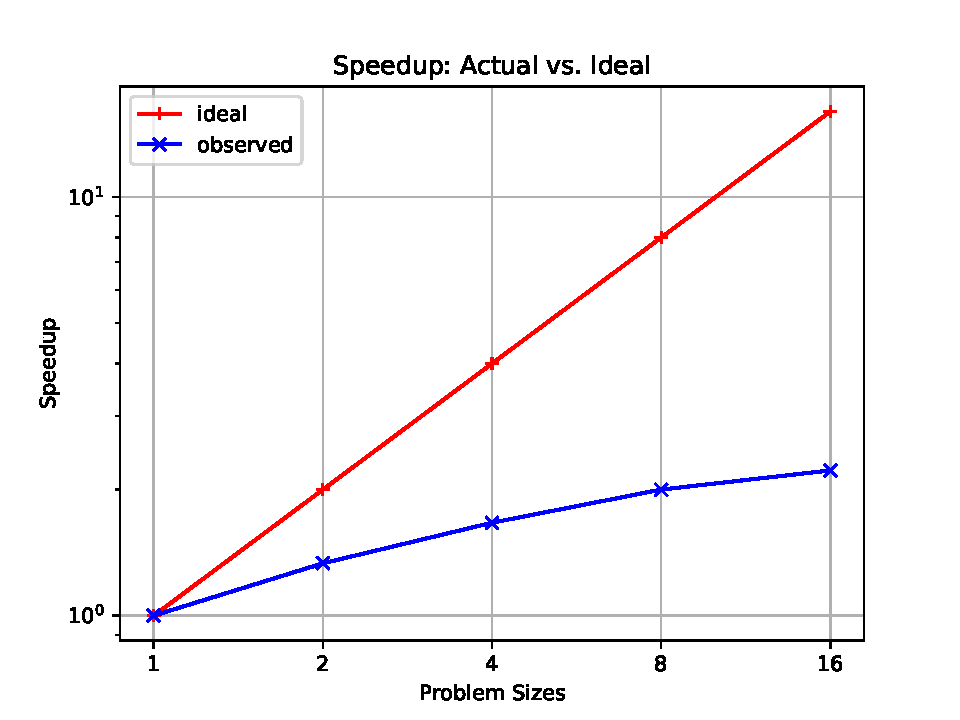
\includegraphics[width=0.45\textwidth]{Figure_1.pdf}
    \caption{Comparison of actual vs. ideal speedup with increasing problem sizes. In this case, we see the observed speedup is quite different than the ideal speedup. Try changing the vertical axis to log-scaling in the Python script that generates the chart. This figure was produced by the sample \texttt{plot\_speedup.py} file.}
    \label{fig:my_label}
\end{figure}





%% if specified like this the section will be committed in review mode
\acknowledgments{
The authors wish to thank A, B, C. This work was supported in part by
a grant from XYZ.
\textit{Comment:} you don't need this section in homework assignments, but you will need it when you create a final, camera-ready version of a technical paper for publication.
}

%\bibliographystyle{abbrv}
\bibliographystyle{abbrv-doi}
%\bibliographystyle{abbrv-doi-narrow}
%\bibliographystyle{abbrv-doi-hyperref}
%\bibliographystyle{abbrv-doi-hyperref-narrow}

\bibliography{template}
\end{document}
